% !TEX encoding   = UTF8
% !TEX spellcheck = ru_RU
% !TEX root = ../seminars.tex

%%==============================
\chapter{Архитектура компьютера}
%%==============================

%%===============================
\section{Архитектура фон Неймана}
%%===============================
\noindent
\begin{minipage}{0.4\columnwidth}
  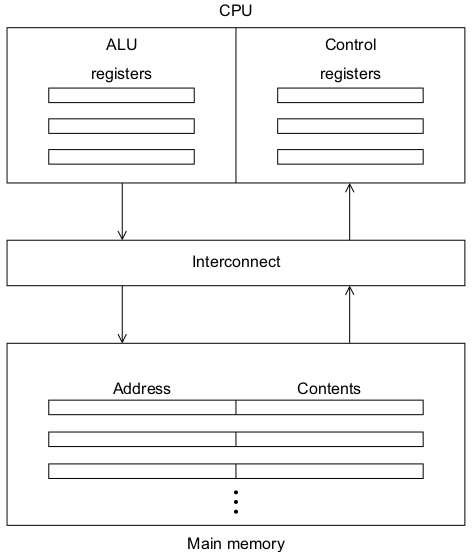
\includegraphics[width=\columnwidth]{images/von_neumann_architecture.png}
\end{minipage}\hfill
\begin{minipage}{0.5\columnwidth}
\parindent=2.5em
\textit{Центральный процессор} (ЦП), или \textenglish{central processor unit} (CPU), "--- это мозг компьютера. Его задача "--- выполнять программы, расположенные в~основной памяти. Он вызывает команды из~памяти, определяет их тип, а затем выполняет одну за~другой. Компоненты соединены \textit{шиной} (\textenglish{bus}), представляющей собой набор параллельно связанных проводов, по~которым передаются адреса, данные и сигналы управления. Шины могут быть внешними (связывающими процессор с~памятью и устройствами ввода--вывода) и внутренними.

Системы RISC (\textenglish{Reduced Instruction Set Computer}) и CISC (\textenglish{Complex Instruction Set Computer}).
\end{minipage}



%%========================================
\section{Процессы, многозадачность и нити}
%%========================================
\textit{Операционная система}~(ОС) "--- существенная часть программного обеспечения, задача которого управлять аппаратными и программными ресурсами компьютера.

Когда пользователь запускает программу, операционная система создаёт \textit{процесс} "--- копию программы, которая может быть выполнена. Он состоит из~нескольких элементов:
\begin{itemfeature}
  \item Код на~машинном языке.
  \item Блок памяти, которая будет включать исполняемый код, \textit{стек вызовов} (\textenglish{call stack}), динамически распределяемую память (кучу, \textenglish{heap}) и некоторые другие части.
  \item Дескрипторы ресурсов, которые операционная система выделяет для~процесса.
  \item Права доступа "--- информация, определяющая какие аппаратные и программные ресурсы доступны данному процессу.
  \item Информация о~состоянии: готов ли процесс к~выполнению или ожидает ресурс, содержимое регистров, распределение занимаемой памяти.
\end{itemfeature}

Большинство современных операционных систем \textit{многозадачные} (\textenglish{multitasking}). Это означает, что они обеспечивают поддержку одновременного выполнения нескольких программ (даже на~одном ядре). После того, как одна запущенная программа отработала небольшой интервал времени (несколько миллисекунд), называемый \textit{квантом} (\textenglish{time slice}), операционная система может запустить другую программу.

Если в~многозадачной ОС процесс ожидает ресурса, то он \textit{блокируется} (\textenglish{block}). Это означает, что его выполнение приостанавливается, и операционная система может запустить другой процесс. \textit{Нити} (\textenglish{threading}) исполнения обеспечивают механизм для~разделения программы на~более или менее независимые задачи так, что когда одна нить блокируется, другая может выполняться. Нить создаётся внутри процесса и разделяет большую часть его ресурсов. Два наиболее важных исключения "--- счётчик команд и стек вызовов. Поэтому создание и переключение между нитями происходит быстрее, чем между процессами.



%%======================================
\section{Модификации модели фон~Неймана}
%%======================================
\vspace{-1em}\begin{flushleft}
  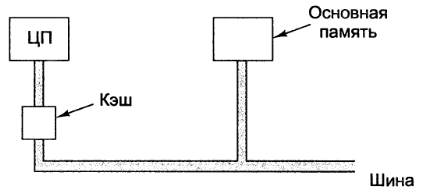
\includegraphics[width=0.45\columnwidth]{images/cache.png}\hfill%
  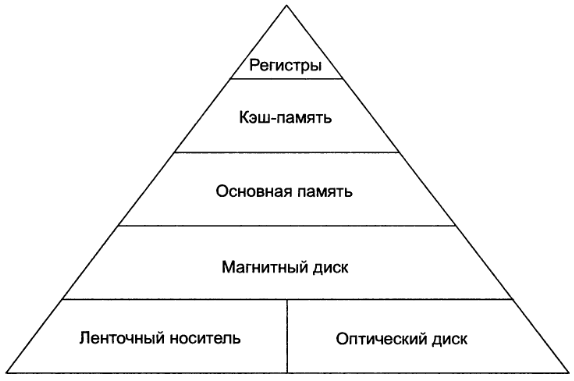
\includegraphics[width=0.45\columnwidth]{images/memory.png}
\end{flushleft}



%%================================
\subparagraph{Основы кэширования.}
%%================================
Кэш-память, или \textit{кэш}~(\textenglish{cache}), "--- набор блоков памяти, обращение к~которым может быть выполнено за~меньшее время, чем к~основной памяти.

С~появлением кэша, сразу возникает вопрос, какие данные и инструкции следует там хранить. В~основе универсальной стратегии лежит идея, что программа стремится использовать данные и инструкции, которые физически расположены рядом с~теми, что использовались недавно. Эту стратегию часто называют \emph{принципом локальности}. За~обращением по~некоторому адресу для~извлечения инструкции или данных в~следующий момент (\emph{временная} локальность) обычно происходит обращение к~соседнему адресу (\emph{пространственная} локальность). Ярким примером служит работа с~массивами.

Для~реализации принципа локальности на~практике система использует \emph{шину}, или соединительные провода, достаточно большой ширины. То есть при~обращении к~памяти в~действительности происходят операции с~блоками данных и инструкций, которые называют \emph{кэш-блоками} или \emph{строками кэша}.

Концептуально, зачастую удобно думать о~кэше ЦП, как о~единой структуре. Однако на~практике его обычно разделяют на~\emph{уровни}: первый уровень~(L1) самый маленький и самый быстрый, более высокие уровни~(L2, L3, \ldots) больше и медленнее.

Когда центральному процессору необходимо загрузить инструкции или данные, он просматривает кэш: в~начале проверяет первый уровень, затем второй и т.\,д. Если необходимая информация найдена, это называют \textit{кэш-попаданием} (\textenglish{cache hit}). А если нет, то это \textit{кэш-промах} (\textenglish{cache miss}), и процессор обращается к~основной памяти, что может приостановить выполнение текущей программы до~тех пор, пока не~будут получены данные.

Для~измерения эффективности вводят \emph{коэффициент кэш-попаданий}~\(h\) (\textenglish{hit ratio}), который показывает соотношение числа обращений к~кэш-памяти и общего числа всех обращений к~памяти, и \emph{коэффициент кэш-промахов} (\textenglish{miss ratio}), равный \(1 - h\).

Пусть~\(c\) "--- время доступа к~кэш-памяти, \(m\) "--- время доступа к~основной памяти. Тогда среднее время доступа:
\[
  t_\text{ave} = c + (1 - h)\,m.
\]
Если \(h \rightarrow 1\), то есть все обращения делаются только к~кэш-памяти, то время доступа стремится к~\(c\). С~другой стороны, если \(h \rightarrow 0\), то есть каждый раз нужно обращаться к~основной памяти, то время доступа стремится к~\(c + m\): сначала требуется время~\(c\) для~проверки кэш-памяти (в~данном случае безуспешной), а затем "--- время~\(m\) для~обращения к~основной памяти.

Когда ЦП пишет данные в~кэш, значение в~кэше и основной памяти становятся различными, или \textit{несогласованными} (\textenglish{inconsistent}). Существует два подхода устранить несогласованность. Немедленное обновление значения в~основной памяти называется \textit{сквозной записью} (\textenglish{write-through}). Этот подход обычно гораздо проще реализуется и, к~тому же, более надёжен, поскольку современная память при~ошибке может восстановить своё предыдущее состояние. К~сожалению, при~этом приходится передавать больше данных в~память, поэтому в~сложных проектах стремятся использовать альтернативный подход "--- \textit{отложенную запись} (\textenglish{write-back}). Обновлённые данные в~кэше помечаются как <<грязные>> (\textenglish{dirty}), и когда строка кэша заменяется новой строкой из~памяти, <<грязная>> строка записывается обратно в~память.



%%================================
\paragraph{Отображение кэш-памяти}
%%================================
на~основную память:
\begin{itemfeature}
  \item \textit{полностью ассоциативный} кэш: строка может быть помещена в~любую позицию;
  \item кэш \textit{прямого отображения}: строка связана с~фиксированной позицией определяемой, например, младшими битами адреса в~основной памяти;
  \item \textit{n-входовый ассоциативный} кэш являет собой промежуточный вариант.
\end{itemfeature}



%%=============================
\paragraph{Виртуальная память.}
%%=============================
Современные операционные системы поддерживают одновременную работу множества задач, которые вынуждены разделять ресурс памяти меж собой. Кроме того, необходимо защищать данные и инструкции каждого процесса от~возможного повреждения со~стороны других процессов.

\emph{Виртуальная память} (\textenglish{virtual memory}) разработана так, чтобы основная память могла быть использована как кэш для~вторичного хранилища (обычно в~дисковом пространстве). Она использует принцип пространственной и временной локальности, сохраняя в~основной памяти только активные части запущенных программ; те части, что простаивают, хранятся в~блоке вторичного хранилища, называемом \textit{файлом подкачки} (\textenglish{swap space}). Подобно кэшу, виртуальная память оперирует с~блоками данных и инструкций. Эти блоки обычно называют \emph{страницами} (\textenglish{pages}). Поскольку доступ ко~вторичному хранилищу может быть в~сотни тысяч раз медленнее, чем к~основной памяти, страницы делают относительно большими "--- большинство систем имеют фиксированный размер страниц, который на~данный момент лежит в~диапазоне от~4 до~16\,Кб.

При~компиляции программы используются виртуальные адреса. Когда программа запускается, создаётся \emph{таблица страниц} (\textenglish{page table}) для~отображения виртуальных страниц на~физические адреса. Обычно создание таблиц осуществляет операционная система, что позволяет гарантировать, что участки памяти, используемые одним процессом, не~пересекается с~памятью других процессов.

Недостаток использования таблиц в~удвоении времени доступа к~основной памяти (обращение к~таблице плюс обращение в~память по~целевому физическому адресу). Для~решения этой проблемы процессоры содержат специальный кэш для~преобразования адресов, называемый \emph{буфером быстрого преобразования} (\textenglish{translation-lookaside buffer, TLB}).

Вследствие медленной работы диска виртуальная память всегда использует отложенную запись, если страница была изменена в~процессе работы программы. А управление таблицой страниц и обращением к~диску можно поручить операционной системе (совместно с~аппаратным обеспечением).



%%=====================================================
\paragraph{Параллелизм выполнения на~уровне инструкций}
%%=====================================================
позволяет улучшить производительность процессора за~счёт разделения на~компоненты, или \emph{функциональные блоки} (\textenglish{functional units}), одновременно выполняющие инструкции.

Существует два основных подхода:
\begin{itemfeature}
  \item \emph{конвейер} (\textenglish{pipeline}), принцип работы схож с~заводским конвейером;
  \item \emph{суперскалярная архитектура} (\textenglish{superscalar architecture}), один конвейер с~большим количеством функциональных блоков.
\end{itemfeature}

\begin{center}
  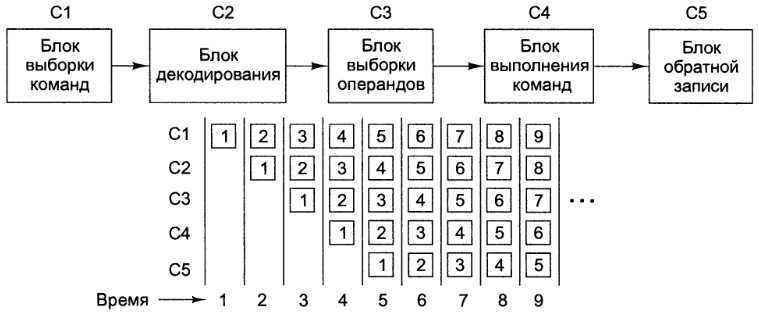
\includegraphics[width=0.7\columnwidth]{images/pipeline.png}
\end{center}



%%=============================================
\paragraph{Многонитевое аппаратное обеспечение}
%%=============================================
предоставляет средства для~продолжения выполнения полезной работы, когда задача, выполняющаяся в~данный момент, была приостановлена, например, в~ожидании загрузки данных из~памяти. В~этот момент, возможно, имеет смысл просто запустить другую нить. Конечно, для~этого система должна поддерживать очень быстрое переключение между нитями.



%%===========================================
\section{Параллельное аппаратное обеспечение}
%%===========================================
Суперскалярную архитектуру и конвейер также можно рассматривать как параллельное аппаратное обеспечение, поскольку функциональные блоки дублируются. Однако, эта форма параллелизма обычно не~видна программисту, и её можно рассматривать как расширение исходной модели фон~Неймана. Под~\emph{параллельным обеспечением} будем понимать обеспечение, которое требует от~программиста изменений в~исходном коде.



%%=======================
\paragraph{SIMD системы.}
%%=======================
\textenglish{Single Instruction-stream Multiple Data-stream}:
\begin{itemfeature}
  \item \emph{векторные процессоры} (\textenglish{vector processors});
  \item \emph{графические процессоры} (\textenglish{graphics processing units, GPU})
\end{itemfeature}



%%=======================
\paragraph{MIMD системы.}
%%=======================
\textenglish{Multiple Instruction-stream Multiple Data-stream}:

\medskip\noindent
\begin{minipage}[c]{0.5\textwidth}
\parindent=2.5em

\begin{itemfeature}
  \item \emph{системы с~общей памятью} (\textenglish{shared-memory systems}), используют один или более многоядерных процессоров, связанных с~единой памятью. Выделяют системы с~\emph{однородным доступов к~памяти} (\textenglish{uniform memory access, UMA}) и \emph{неоднородным доступом к~памяти} (\textenglish{nonuniform memory access, NUMA});
\end{itemfeature}

\end{minipage}\hfill\begin{minipage}{0.45\textwidth}

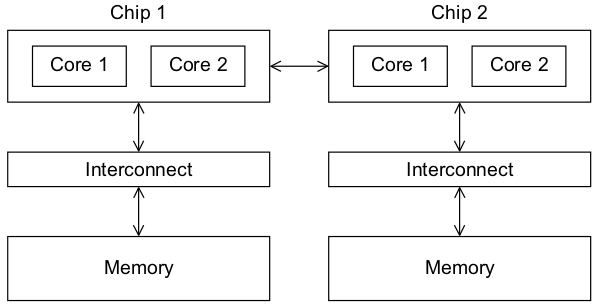
\includegraphics[width=\columnwidth]{images/numa_multicore_system.png}

\end{minipage}

\begin{itemfeature}
  \item \emph{системы с~распределённой памятью} (\textenglish{distributed-memory systems}). Обычно \emph{узлами} (\textenglish{nodes}) таких систем являются системы с~общей памятью, поэтому их иногда называют \emph{гибридными} (\textenglish{hybrid systems}). \emph{Глобальная сеть} (\textenglish{grid}) обеспечивает инфраструктуру, необходимую для~объединения больших сетей географически распределённых компьютеров в~одно целое. В~общем, такие системы будут \emph{гетерогенными} (\textenglish{heterogeneous}), то есть индивидуальные узлы могут иметь разную архитектуру.
\end{itemfeature}



%%===============
\ExercisesSection
%%===============
Рассмотрим влияние кэширования на~производительность программы. Для~этого создадим структуру данных, которая хранит целочисленный идентификатор и массив символов фиксированного размера.

\cppfile[firstline=13, lastline=19]{projects/sem14/cache.cpp}



%%============================
\paragraph{Тестовая оснастка.}
%%============================
Напишем функцию, которая создаёт тестовый массив заданного размера, заполняя поле \code{id} элементов псевдослучайными значениями в~диапазоне от~\code{0} до~\code{high}.

\cppfile[firstline=22, lastline=36]{projects/sem14/cache.cpp}

\noindent Здесь используются возможности стандартной библиотеки \code{<random>}. При~желании, можно выбрать другое распределение, отличное от~равномерного. Обратим внимание на~пустые скобки при~указании шаблонного типа. Объявление класса выглядит примерно так:

\begin{minted}[linenos=false, fontsize=\small]{c++}
template<class IntType = int>
class uniform_int_distribution;
\end{minted}

\noindent Видно, что параметр по~умолчанию "--- тип \code{int}. Именно поэтому мы можем его не~указывать явно. А угловые скобки говорят о~том, что это шаблон.

Напишем тестовую функцию, которая запускает два различных варианта упорядочивания элементов в~массиве заданного размера и измеряет время выполнения каждого алгоритма. Добавим проверку, что оба варианта приводят к~одинаковому порядку. В~качестве таймера можно использовать класс-обёртку \code{Timer}, описание которого приведём ниже.

\cppfile[firstline=80, lastline=101]{projects/sem14/cache.cpp}

Функцию \code{main()} нашей тестовой программы можно записать следующим образом:

\cppfile[firstline=104, lastline=104]{projects/sem14/cache.cpp}
\cppfile[firstline=106, lastline=115]{projects/sem14/cache.cpp}



%%===============================
\paragraph{Класс \texttt{Timer}.}
%%===============================
Это небольшой класс-обёртка, использующий стандартную библиотеку \code{<chrono>}. Его реализация проста и очевидна, не~требует дополнительных комментариев. Код следует разместить в~файле \code{timer.h} и подключить к~коду остальной тестовой оснастки.

\cppfile[firstline=7, lastline=30]{projects/sem14/timer.h}

Теперь рассмотрим первый вариант сортировки. Упорядочивать будем по~полю \code{id}. Положим, что элементы массива достаточно велики, чтобы пренебречь временем копирования при~обменах. Для~решения этой проблемы создадим массив указателей и упорядочим его. (В~случае необходимости легко получить новый, упорядоченный, массив исходных элементов, используя указатели.)

\cppfile[firstline=39, lastline=51]{projects/sem14/cache.cpp}

Второй вариант сделаем чуть хитрее. Добавим вспомогательный массив пар \code{(указатель, id)} и выполним упорядочивание без~косвенного доступа к~исходным элементам.

\cppfile[firstline=54, lastline=77]{projects/sem14/cache.cpp}

Проведите серию запусков программы и постройте несколько графиков подобных тем, что приведены на~рисунке~\ref{fig:caching}.

\begin{figure}[h]
  {\centering
    \hfill
    \subbottom[в~зависимости от~количества элементов\label{fig:caching:a}]{%
      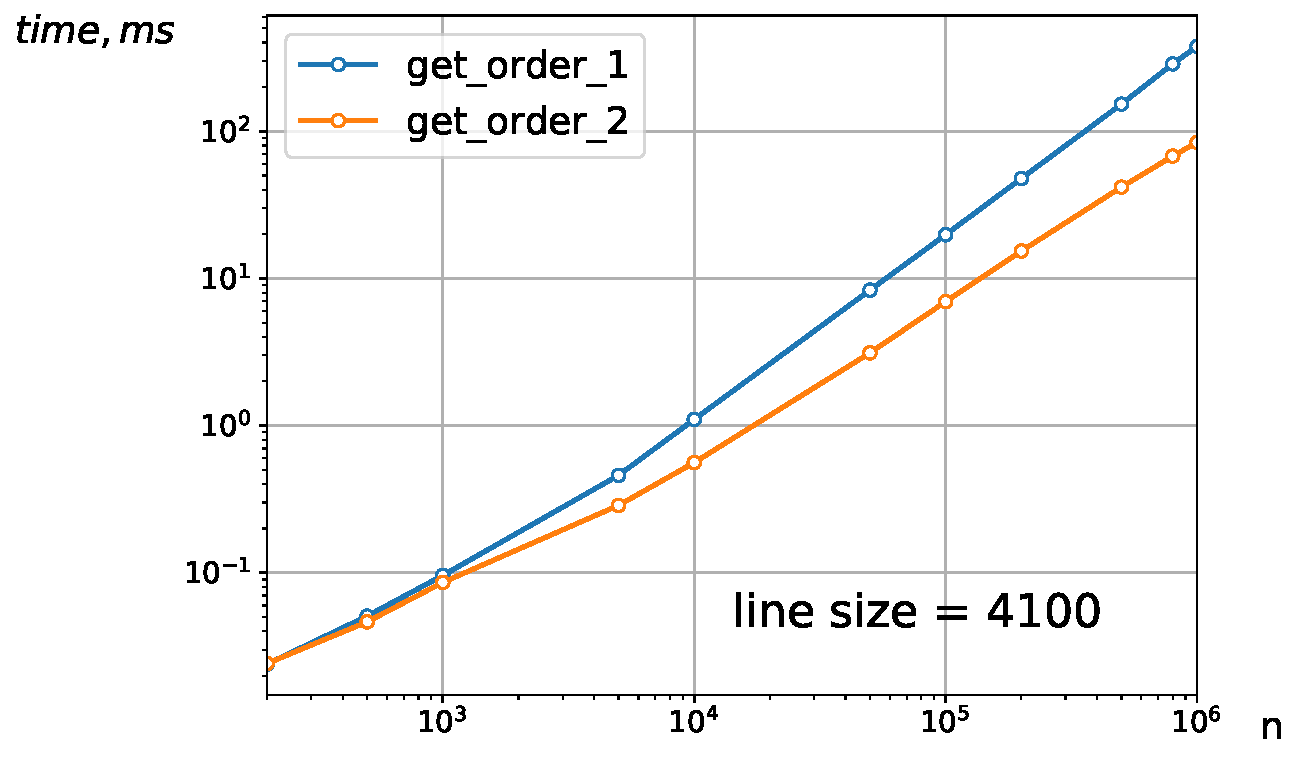
\includegraphics[width=0.45\columnwidth]{images/cache_impact_by_n.pdf}}
    \hfill
    \subbottom[в~зависимости от~размера самого элемента\label{fig:caching:b}]{%
      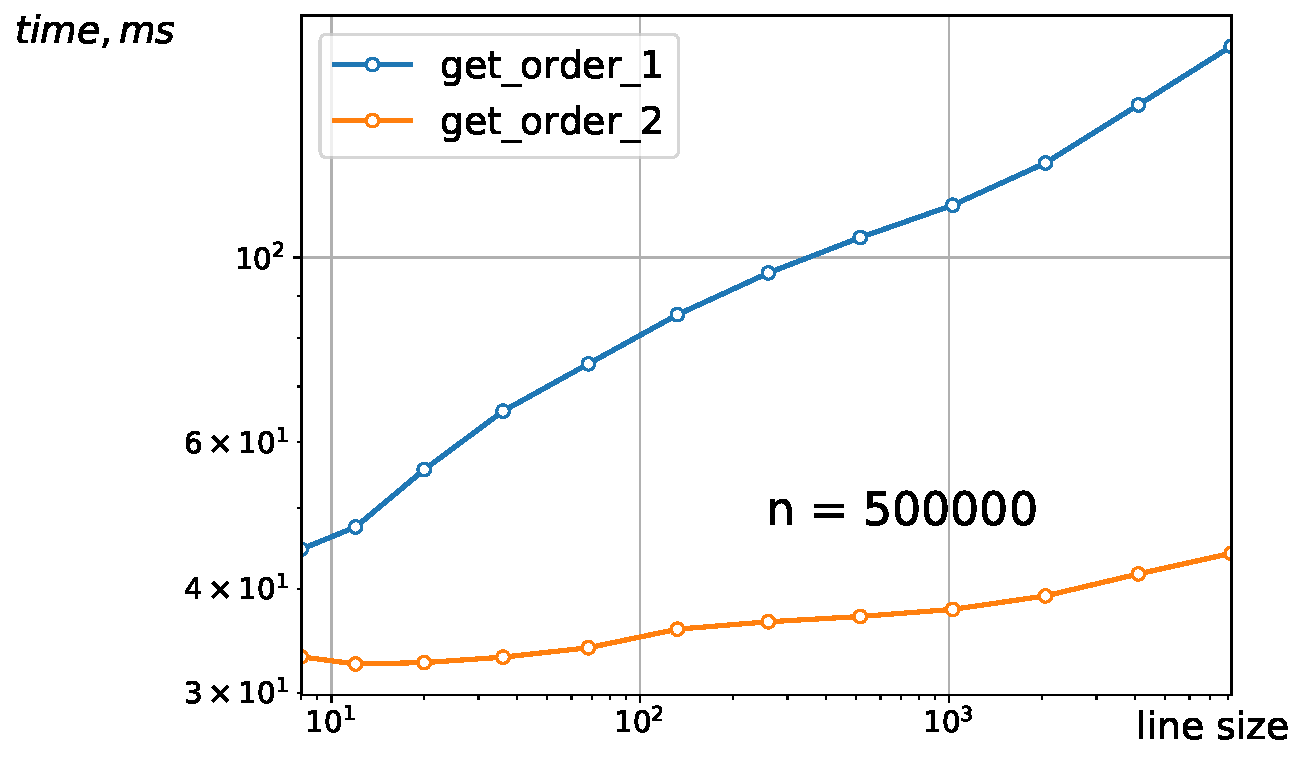
\includegraphics[width=0.45\columnwidth]{images/cache_impact_by_line_size.pdf}}
    \hfill
    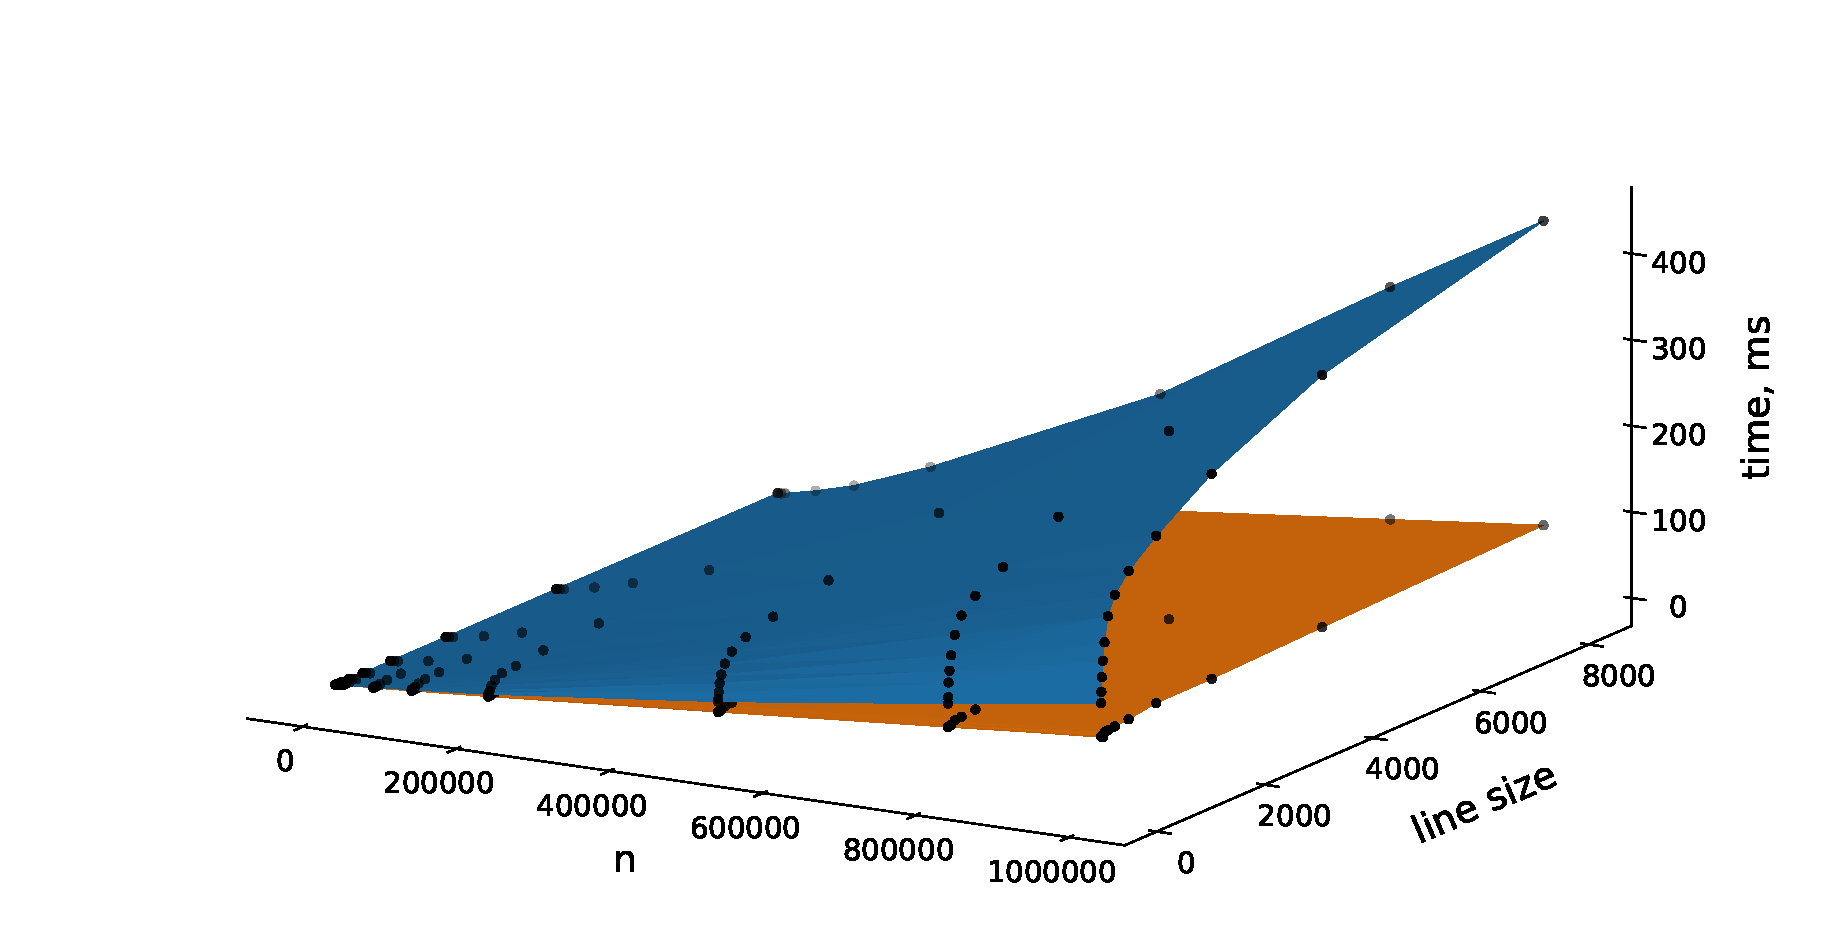
\includegraphics[width=0.7\columnwidth]{images/cache_impact.pdf}

  }
  \caption{Влияние кэширования на~производительность программы.}
  \label{fig:caching}
\end{figure}

Объясните полученное поведение кривых. Используйте знания об~устройстве и работе кэша, изложенные выше.



%%================
\WhatToReadSection
%%================
\begin{tabular}{@{}l@{}}
  \citeauthor[глава~3, стр.~390--398]{Harris:2015:ru} \\
  \citeauthor[глава~7, стр.~1091--1131; глава~8, стр.~1163--1240]{Harris:2015:ru} \\
  \citeauthor[глава~2, стр.~15--46]{Pacheco:2011:en}
\end{tabular}
